\documentclass[14pt]{article}
\usepackage[utf8]{vietnam}
\usepackage{graphicx}
\usepackage{listings}
\graphicspath{ {figures/} }
\usepackage{fancyhdr}
\usepackage{geometry}
\usepackage{float}
\usepackage[bottom]{footmisc}
\usepackage{afterpage}
\usepackage{multirow}
\usepackage[table]{xcolor}
\definecolor{highlight}{RGB}{230, 230, 230}
%\newcommand{\kb}{\textit{KB/s}}
%\newcommand{\kbs}{\textit{Kbps}}
%\newcommand{\mbs}{\textit{Mbps}}
%\newcommand{\gbs}{\textit{Gbps}}
%\newcommand{\mb}{\textit{MB/s}}
\newcommand{\sep}{\rule{\textwidth}{0.007pt}\\}
%\newcommand{\sep}{\vspace{0.5cm}}
\lstset{numbers=left, numberstyle=\tiny, stepnumber=2, numbersep=5pt, tabsize=2, language=java, basicstyle=\small}
\newcommand\blankpage{%
    \null
    \thispagestyle{empty}%
    \addtocounter{page}{-1}%
    \newpage}
\geometry{
	left=2cm, right=2cm,
	top=2cm, bottom=2cm,
	includefoot=true,
	includehead=true,
	headsep = 40pt,
}
% create the header for this file
\pagestyle{fancy}
\begin{document}
\thispagestyle{empty}


\fancyhead{} % clear all header fields
\fancyhead[L]{
 \begin{tabular}{rl}
    \begin{picture}(25,15)(0,0)
    \put(0,-8){
\includegraphics[width=8mm, height=8mm]{Images/hcmut.pdf}}
   \end{picture}&
	\begin{tabular}{l}
		\textbf{\bf Đại học Bách Khoa Tp. Hồ Chí Mính}\\
		\textbf{\bf Khoa Khoa học \& Kỹ thuật Máy Tính}
	\end{tabular} 	
 \end{tabular}
}

\fancyfoot{} % clear all footer fields
\fancyfoot[L]{\scriptsize Báo cáo bài tập lớn số 2}
\fancyfoot[R]{\scriptsize \thepage}
\renewcommand{\headrulewidth}{0.3pt}
\renewcommand{\footrulewidth}{0.3pt}

\begin{center}
\LARGE\bfseries ĐẠI HỌC QUỐC GIA TP HỒ CHÍ MINH \\
TRƯỜNG ĐẠI HỌC BÁCH KHOA \\

\end{center}
\begin{center}
\LARGE\bfseries 
Khoa Khoa Học \& Kỹ Thuật Máy Tính
\end{center}
\begin{center}

\includegraphics[scale=0.2]{Images/hcmut.pdf}\\[1cm]
\end{center}

\vspace{1cm}

\begin{flushleft}
\Large \bfseries TRÍ TUỆ NHÂN TẠO\\
Bài tập lớn số 2\\[0.5cm]
\end{flushleft}
\rule{\textwidth}{1pt}
\vspace{2pt}
\begin{center}
\huge
\begin{tabular}{@{}l}
ROBOCODE\\[10pt]
\end{tabular}
\end{center}
\rule{\textwidth}{1pt}\\[1cm]

\vspace{1cm}

\begin{minipage}[t]{0.60\linewidth}
\textbf{GVHD}: \\
Gs. Cao Hoàng Trụ\\
Ths. Vương Bá Thịnh

\end{minipage}
\begin{minipage}[t]{0.25\linewidth}
\textbf{NHÓM Feederz:}\\
Nguyễn Kim Trung Hiếu\\
Đỗ Nguyễn Khánh Hoàng\\
\end{minipage}
\begin{minipage}[t]{0.20\linewidth}
\textbf{}\\
51201097\\
51201200\\
\end{minipage}
\begin{center}

\vspace{2cm}
{Tp. HCM, 05/2015}

\end{center}

%\newpage
%\thispagestyle{empty}
%\emph{ }
\newpage
\thispagestyle{empty}
\tableofcontents
\thispagestyle{empty}

\newpage
\thispagestyle{empty}
\listoffigures

%\newpage
%\thispagestyle{empty}
%\begin{center}
%This page intentionally left blank
%\end{center}
\newpage
\section{Robocode}
\subsection{Giới thiệu}
Robocode là một chương trình trò chơi mà mục tiêu là tạo ra một robot, các robot mô phỏng xe tăng trong một đấu trường chiến đấu để tìm và cạnh tranh với các robot khác, nó được trang bị với hệ thống radar. Một robot có thể di chuyển tới, lui ở các tốc độ khác nhau và di chuyển qua trái, qua phải. Các radar và tháp pháo có thể được chuyển sang trái hoặc sang phải độc lập với nhau so với phần còn lại của xe tăng. Khẩu súng có thể bắn. Khi cài đặt một trận đấu, ta có thể xem được trận đấu từ bên ngoài màn hình chơi hoặc dùng máy tính mô phỏng trận đấu mà không cần hiển thị đồ họa. Người chơi là các lập trình của robot, những người này sẽ không ảnh hưởng trực tiếp vào trò chơi mà thay vào đó người chơi phải lập trình làm sao cho robot thông minh có thể xử lý và phản ứng tất cả các sự kiện xảy ra trong lĩnh vực chiến đấu. Khi một robot đối thủ lọt vào rađa, một sự kiện sẽ được sinh ra và một hành động phù hợp sẽ được robot thực hiện. Robot có thể lấy được các thông tin về một đối thủ đang trong vùng quét của ra đa như tốc độ, heading, năng lượng còn lại, tên và gốc giữa heading của nó với robot đối thủ, khoảng cách giữa nó với đối thủ. Dựa vào các thông tin này mà rô bốt sẽ đưa ra các hành động phù hợp. Ví dụ, khi phát hiện một đối thủ trong vòng rađa, robot có thể dùng súng để bắn. Các robot có thể ra trận cùng với đội robot của nó. Bằng việc giao tiếp với các robot khác, chúng có thể trao đổi các thông tin như nơi có đối thủ được phát hiện và dựa trên chiến lược được chọn, một robot có thể chạy trốn từ đám các đối thủ hoặc thông báo tin cho các đồng minh của nó về thông tin các đối thủ đó. Các robot được viết bằng ngôn ngữ lập trình Java và các trò chơi Robocode có thể chạy trên bất kỳ hệ điều hành được hỗ trợ bởi các nền tảng Java, bao gồm tất cả các hệ thống phổ biến như Windows, Mac OS X, Linux etc.
\subsection{Sơ lược về robot của nhóm (Feederz)}
Về cơ bản, một robot chủ yếu có 2 hành động chính: di chuyển sao cho ít trúng đạn nhất, và ngắm bắn sao cho chính xác nhất. Có rất nhiều kỹ thuật trong việc điều khiển này, ví dụ:
- Di chuyển: đứng yên, di chuyển theo đường thẳng, theo vòng tròn, theo pattern, di chuyển ngẫu nhiên, wave surfing...
- Ngắm bắn: bắn trực tiếp, dự đoán theo đường thẳng, theo hình tròn, pattern matching, guess factor, dynamic clustering...
Robot của nhóm sử dụng 2 kỹ thuật khá thông dụng trong việc điều khiển di chuyển và ngắm bắn, đó là Wave Surfing (di chuyển) và Guess Factor Targeting (ngắm bắn).
Do vấn đề thời gian nên nhóm chỉ hiện thực một cách khá đơn giản 2 kỹ thuật này. Sẽ còn rất nhiều cách để tăng tính hiệu quả của robot.

\section{Tổ chức Class}
Chương trình được tổ chức rõ ràng với 04 class chính. Nhiệm vụ mỗi class được phân chia cụ thể và hợp lý.
\begin{figure}[H]
\centering
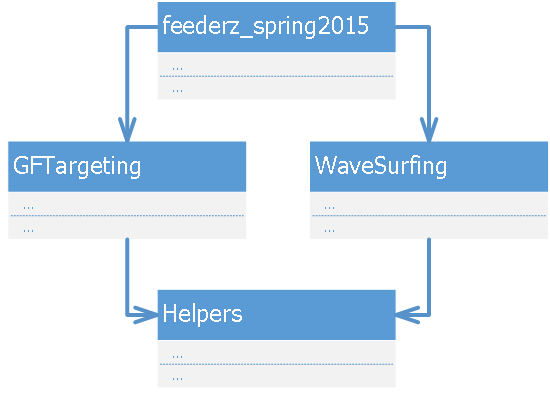
\includegraphics[scale=0.5]{images/classStructrure.png}
\caption{Tổ chức class}
\end{figure}
\begin{itemize}
	\item \textbf{feederz\_spring2015}: class chính hiện thực robot. Ở đây chứa các hàm cơ bản mà hệ thống sẽ gọi trong suốt quá trình robot chạy
	\item \textbf{WaveSurfing}: class hiện thực kỹ thuật Wave Surfing, chịu trách nhiệm tính toán và điều khiển đường đi của robot, né đạn và né tường
	\item \textbf{GFTargeting}: class hiện thực kỹ thuật Guess Factor, chịu trách nhiệm tính toán và điều khiển súng của robot để nhắm chính xác mục tiêu
	\item \textbf{Helpers} class chứa các hàm bổ trợ được sử dụng bởi các class trên
\end{itemize}
\section{Kỹ thuật Wall Smoothing}
Theo luật của robocode, mỗi lần va chạm với tường robot cũng bị mất năng lượng giống như khi bị trúng đạn. Hơn nữa, nếu robot va chạm với tường và mắc kẹt ở một trong bốn góc của sân đấu thì khả năng bị tiêu diệt sớm lại càng cao hơn. Do vậy, để nâng cao khả năng sống còn của robot, việc đầu tiên cần nghĩ ngay tới đó là làm cho robot "né" được tường trong lúc chiến đấu, đừng để nó di chuyển vào những điểm chết hoặc những điểm quá gần tường.

Đầu tiên ta thiết lập một vùng an toàn cho robot. Trong suốt trận đấu, ta cố gắng điều khiển cho robot di chuyển không vượt qua giới hạn của vùng này. Cụ thể, kích thước vùng này được quy định bởi một hình chữ nhật \textit{playingRectangle} như trong source code.
\begin{lstlisting}[caption = Thiết lập vùng an toàn, frame = single]
public static final int BATTLEFIELD_WIDTH = 8100;
public static final int BATTLEFIELD_HEIGHT = 600;
static final int BOUNDARY_SIZE = 18;
public static Rectangle2D.Double playingRectangle = new Rectangle2D.Double(
		BOUNDARY_SIZE, BOUNDARY_SIZE,
		BATTLEFIELD_WIDTH - BOUNDARY_SIZE * 2, 
		BATTLEFIELD_HEIGHT - BOUNDARY_SIZE * 2);
\end{lstlisting}
Kích thước cố định của sân đấu là $800 \times 600$. Vùng an toàn là hình chữ nhật nhỏ bên trong, cách biên của sân đấu một khoảng BOUNDARY\_SIZE = 18.

Xử lý va chạm với tường được giải quyết bằng kỹ thuật Wall Smoothing. Giải thuật này cố gắng tìm ra một góc gọi là "an toàn", nghĩa là nếu robode tiến theo góc đó thì nó không thể va chạm với tường đồng thời cũng không di chuyển quá gần về phía đối thủ.
\begin{lstlisting}[caption = wallSmoothing function, frame = single]
public double wallSmoothing(Point2D.Double botLocation, double angle,int orientation) {
	Point2D.Double guesingPosition = 
									Helpers.getPositionFromAngleAndDistance(botLocation, angle, WALL_STICK);
	while (!playingRectangle.contains(guesingPosition)) {
		angle += orientation * 0.05;
		guesingPosition = Helpers.
			getPositionFromAngleAndDistance(botLocation, angle, WALL_STICK);
	}
	return angle;
}
\end{lstlisting}
Hàm wallSmoothing cần biết 03 thông tin để có thể xác định được góc đi an toàn tiếp là góc nào. Chúng là:
	\begin{itemize}
		\item Vị trí hiện tại của robot
		\item Góc đi vuông góc. Thật khó trình bày bằng lời góc này xác định như thế nào. Tuy nhiên nhiên nếu nhìn vào hình vẽ ta thấy, để đi vuông góc với phương nối giữa robot và enemy, robot phải đi theo hướng $P_1$. Và góc \textit{angle} chính là góc tương đối giữa mũi tên $P_1$ với trục đứng chỉ $0^o$, tức góc $\alpha$. Vì góc này nằm bên trái trục $0^o$ nên nó sẽ có giá trị âm.
		\item Hướng di chuyển hiện tại. Nếu chọn enemy làm tâm thì robot có 02 hướng chính để di chuyển là theo chiều kim đồng hồ và ngược chiều kim đồng hồ tướng ứng với giá trị +1 và -1 của \textit{orientation}. Như trong hình vẽ, robot đang di chuyển theo hướng thuận chiều kim đồng hồ nên giá trị này sẽ là +1.
	\end{itemize}
Để hiểu rõ cách hoạt động của giải thuật này, ta sẽ xét trường hợp trong hình. Theo đó nếu đi theo góc $\alpha$ thì sau một đoạn đường WALL\_STICK = 160, vị trí của robot là $P_1$ - tức nằm trong vùng nguy hiểm. Giải thuật sẽ cố gắng xoay mũi tên này vào sâu trong sân đấu để vị trí mới này nằm trong vùng an toàn, đồng thời góc này phải hướng ra xa enemy lớn nhất có thể. Và do đó, mũi tên này sẽ quay vào trong và dừng lại khi đạt góc $\beta$ tương ứng với vị trí $P_2$. Cứ như vậy, giải thuật sẽ luôn hướng góc di chuyển của robot vào trong sân đấu và giữ khoảng cách an toàn đối với tường.
\begin{figure}[H]
\centering
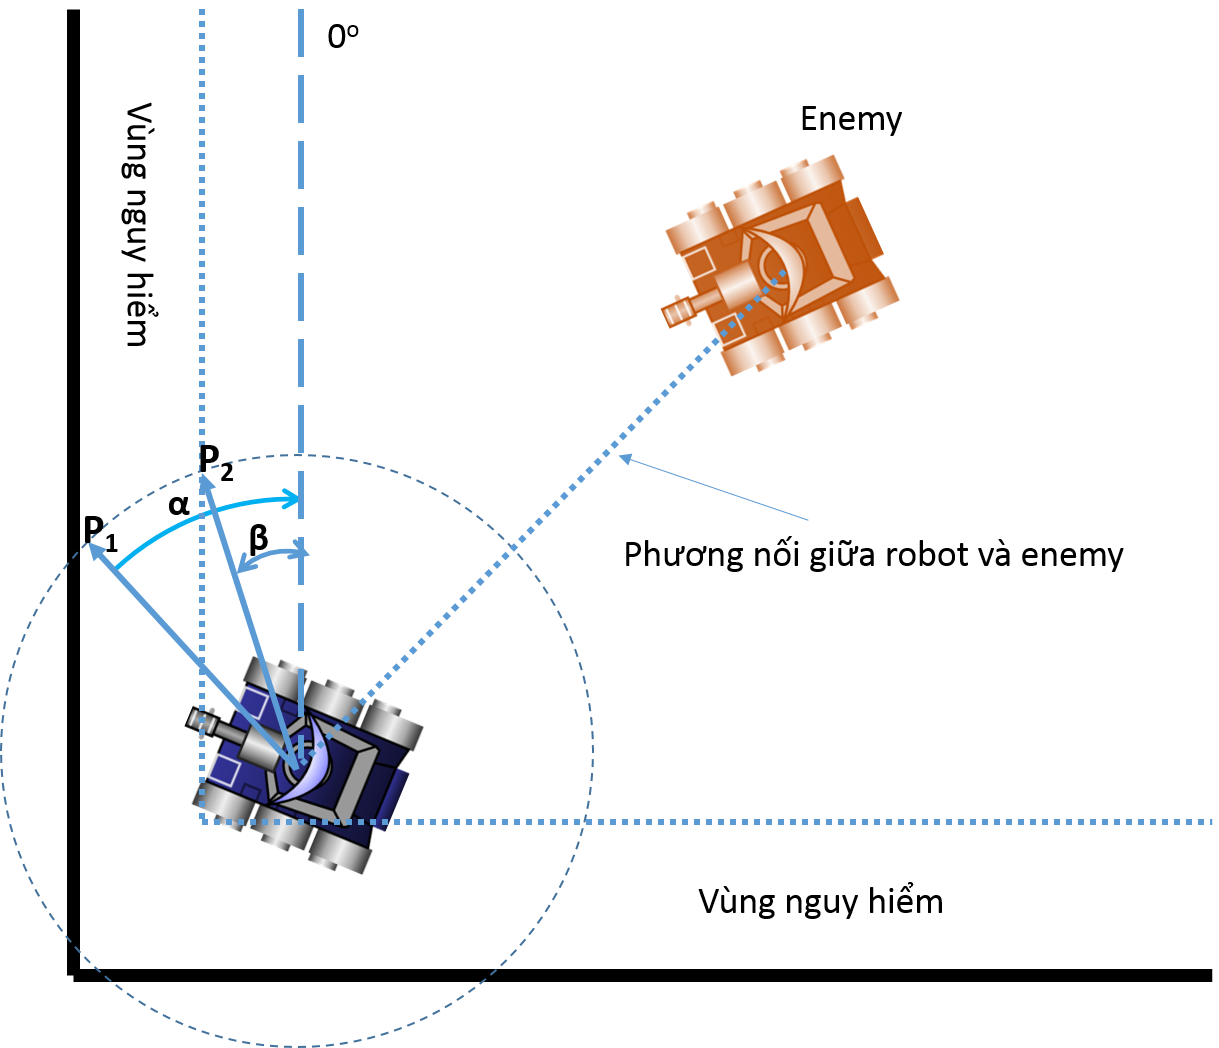
\includegraphics[scale=0.5]{images/wallsmoothing.png}
\caption{Kỹ thuật Wall Smoothing}
\end{figure}
\section{Kỹ thuật Wave Surfing}
\subsection{Giới thiệu}
Một đội chơi đến từ Bồ Đào Nha tên là ABC là những người đầu tiên mang kỹ thuật Wave Surfing vào sử dụng khi họ áp dụng để phát triển robot Shadow vào giữa năm 2004. Cho đến tháng 4 năm 2010, top 40 đội đứng đầu đều sử dụng những dạng biến thể của nó để phát triển robot cho mình. Mấu chốt của kỹ thuật này đó là việc xác định thời điểm đối phương bắn đạn để từ đó dự đoán mục tiêu của nó. Càng nhiều thông tin thu thập được sau mỗi phát bắn, khả năng dự đoán vùng nguy hiểm, tức vùng mà đối phương thường nhắm vào, càng chính xác hơn, để từ đó lựa chọn những đường đi phù hợp.
\subsection{Trừu tượng hóa thông tin đạn bắn}
Để tiện cho việc quản lý, những thông tin về đạn được thu thập, tổ chức và quản lý theo từng wave. EnemyWave là một đối tượng trừu tượng dùng để đóng gói thông tin một viên đạn bắn ra. Chúng bao gồm:
	\begin{itemize}
		\item fireLocation: vị trí mà ở đó viên đạn được bắn ra.
		\item fireTime: thời điểm bắn đạn
		\item bulletVelocity: vận tốc của viên đạn
		\item directAngle: góc bắn
		\item distanceTraveled: khoảng cách viên đạn đã đi được, tính từ fireLocation
		\item direction: hướng bắn
	\end{itemize}
\begin{lstlisting}[caption = EnemyWave, frame = single]
class EnemyWave {
	Point2D.Double fireLocation;
	long fireTime;
	double bulletVelocity, directAngle, distanceTraveled;
	int direction;

	public EnemyWave() {}
}
\end{lstlisting}
\begin{figure}[H]
\centering
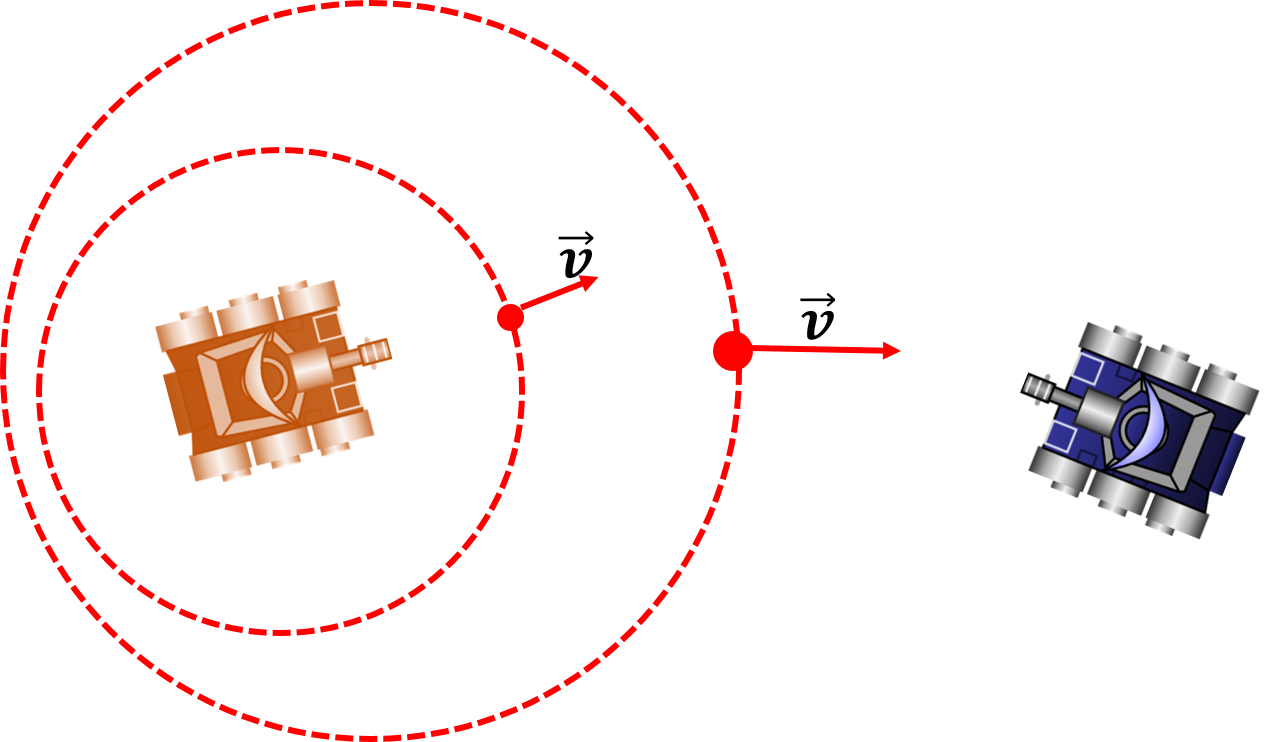
\includegraphics[scale=0.5]{images/wavesurfing_introduction.png}
\caption{EnemyWave}
\end{figure}
\subsection{Nhận biết thời điểm bắn đạn}
API của robocode không cung cấp sự kiện nào để nhận biết việc bắn đạn. Tuy nhiên chúng ta có thể xác đinh được điều này thông qua sự sụt giảm năng lượng của đối phương. Như đã biết, mỗi lần bắn đạn robot sẽ bị mất một khoảng năng lượng và lượng thâm hụt $deltaEnergy$ này thỏa mãn $0 < deltaEnergy \leq 3.0$. Mỗi khi radar phát hiện được đối phương có dấu hiệu này thì chương trình khởi tạo một EnemyWave mới. Việc dự đoán này không phải lúc nào cũng chính xác 100\% và các cải thiện sẽ được trình bày trong những phần sau.
\subsection{Phân chia phạm vi nguy hiểm}
Mỗi khi robot bị trúng đạn, thông tin của viên đạn được truy xuất để phục vụ cho việc phân hoạch vùng nguy hiểm. Việc phân hoạch này có thể dựa trên nhiều yếu tố bao gồm cả vận tốc đạn, khoảng cách đạn hoặc là góc bắn. Tuy nhiên vì chương trình khá đơn giản nên chúng em chỉ hiện thực phân hoạch dựa trên góc bắn. 
\begin{figure}[H]
\centering
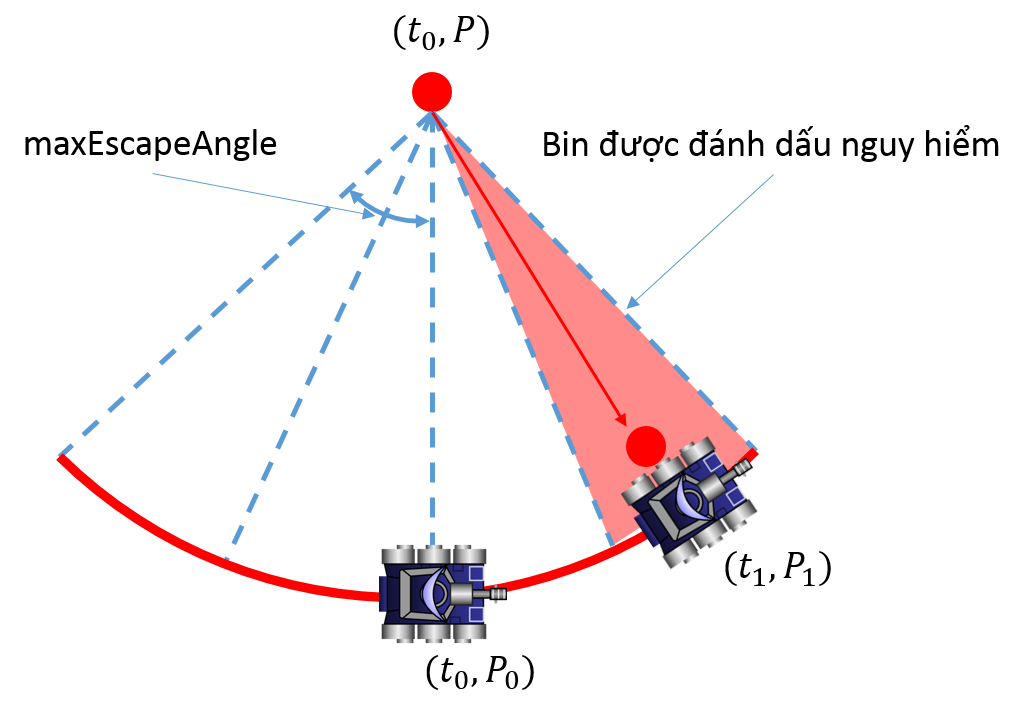
\includegraphics[scale=0.5]{images/segmentation.png}
\caption{Phân hoạch vùng nguy hiểm}
\end{figure}
Theo đó ứng với mỗi EnemyWave, hoặc nói theo cách khác là ứng với mỗi viên đạn được bắn ra, chúng ta sẽ xác định được một góc bắn như hình vẽ. Góc này có độ lớn bằng 2 lần góc maxEscapeAnlge\footnote{Là góc lớn nhất mà robot có thể di chuyển được trong một đơn vị thời gian - một tick. Việc giới hạn này là hợp lý vì mọi góc nằm ngoài khoảng này là không cần xem xét vì robot không thể nào di chuyển tới đó được} và được chia ra thành những phần bằng nhau được gọi là BIN. Trong chương trình sử dụng 47 BIN còn trong hình minh họa thì chia ra được 4 BIN. Một BIN được đánh dấu là nguy hiểm nếu như robot bị trúng đạn khi đang di chuyển trong BIN đó. Chẳng hạn như trong hình vẽ, tại thời điểm $t_0$ robot đang ở vị trí $P_0$ và nhận thấy đối thủ bắn ra viên đạn tại ví trí $P$. Cho đến thời điểm $t_1$ robot bị viên đạn đó đụng phải tại vị trí $P_1$ - thuộc BIN thứ 4. BIN này được tô đỏ trong hình vẽ và nghĩa là trong tương lai, nếu gặp trường hợp tương tự như vậy, robot sẽ hạn chế di chuyển vào BIN này. Tất cả các bị này được tổ chức và lưu trong biến statArray[].

Theo cách đánh dấu như vậy, càng về sau, sự phân hoạch vùng nguy hiểm này sẽ càng chính xác, và robot sẽ học được chiến lược bắn đạn của đối phương để tìm đường đi an toàn cho mình.
\subsection{Kiểm tra mức nguy hiểm}
Mỗi khi nhận biết một viên đạn đang bay tới gần, chương trình sẽ tiến hành kiểm tra xem mức độ nguy hiểm của hướng mình đang đi, nghĩa là xác định xem, nếu cứ tiếp tục đi như vậy thì khả năng viện đạn này va chạm robot cao đến mức nào. Sự đánh giá này dựa trên những thông tin thu thập được từ các BIN trong statArray. Hàm checkDanger sẽ làm công việc đó.
\begin{lstlisting}[caption = checkDanger, frame = single]
public double checkDanger(EnemyWave surfWave, int direction) {
	int index = calculateIndex(surfWave,
			predictPosition(surfWave, direction));
	return statArray[index];
}
\end{lstlisting}
Từ thông tin về viên đạn sắp tới surfWave và hướng đi chuyển hiện tại direction hàm dự đoán vị trí của robot bằng predictPosition và tính toán hệ số của BIN cần tìm. Sau đó trả về giá trị của BIN này trong statArray.
\subsection{Chọn hướng đi an toàn}
Việc lựa chọn này chỉ dựa trên thông tin của viên đạn gần nhất comingWave. Hàm tiến hành kiểm tra mức nguy hiểm của hai hướng đi trái phải (ngược chiều, cùng chiều kim đồng hồ). Sau khi lựa chọn được một hướng đi an toàn nhất, góc tìm được sẽ được xử lý bởi hàm wallSmoothing để tránh trường hợp đụng tường. Góc goAngle trả về là góc cuối cùng mà robot sẽ luôn định hướng đi theo trong suốt chương trình.
\begin{lstlisting}[caption = getPerfectAngleToGo, frame = single]
public double getPerfectAngleToGo() {
	EnemyWave comingWave = getClosestSurfableWave();
	if (comingWave == null) {
		return Double.POSITIVE_INFINITY;
	}
	double dangerLeft = checkDanger(comingWave, -1);
	double dangerRight = checkDanger(comingWave, 1);

	double goAngle = Helpers.getAbsoluteBearingAngle(
			comingWave.fireLocation, ourRobotPosition);
	if (dangerLeft < dangerRight) {
		goAngle = wallSmoothing(ourRobotPosition, goAngle - (Math.PI / 2),
				-1);
	} else {
		goAngle = wallSmoothing(ourRobotPosition, goAngle + (Math.PI / 2),
				1);
	}
	return goAngle;
}
\end{lstlisting}
\subsection{Những biện pháp cải tiến}
{\bf Giữ khoảng cách cố định}\\
Chương trình không quan tâm đến việc giữ khoảng cách tương đối giữa robot và enemy. Nếu cải thiện được thì việc dự đoán đạn của robot sẽ chính xác hơn.\\
{\bf Theo dõi năng lượng của đối thủ chính xác hơn}\\
Như đã trình bày ở phần trước, mỗi lần phát hiện ra đối thủ mất một mức năng lượng $0 < p \leq 3.0$ thì robot sẽ ghi nhận một viện đạn được bắn ra. Cách dự đoán này tuy đa phần chính xác những có một số trường hợp ngoại lệ, đặc biệt là khi gần kết thúc trận đấu - cả hai đều bắn đi những viên đạn có năng lượng nhỏ. Nói là không chính xác bởi vì không phải lúc nào đối thủ mất năng lượng cũng đều do bắn đạn. Đó có thể là do nó bị trúng đạn của ta bắn. Trong trường hợp đó, data thu thập được sẽ bị sai do những "viên đạn ảo" này, ảnh hưởng đến khả năng dự đoán.\\
{\bf Thay đổi chiến lược né đạn}\\
Hiện tại ý tưởng né đạn vẫn là xác định xem viên đạn nào di chuyển đến gần robot nhất để né. Giải pháp này không hiệu quả bằng việc xem xét né viên đạn sẽ chạm robot trước thay vì viên gần nhất.
\section{Kỹ thuật Guess Factor Targeting}
\subsection{Giới thiệu}
\begin{figure}[H]
\centering
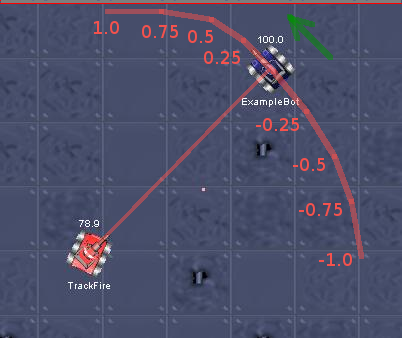
\includegraphics[scale=0.5]{images/GuessFactors.png}
\caption{Guess Factor Targeting}
\end{figure}
Guess Factor Targeting là 1 kỹ thuật ngắm bắn khá đơn giản nhưng cũng không kém phần hữu hiệu được sử dụng trong robocode.
Về cơ bản, vào thời điểm bắn, ta xác định khoảng khu vực mà mục tiêu có thể di chuyển đến, chia chúng ra làm nhiều phần gọi là các BIN \footnote{GuessFactor 0.0 (BIN ở giữa) trỏ trực tiếp tới hướng mục tiêu, GuessFactor 1.0 (BIN đầu tiên) trỏ tới vị trí xa nhất mà mục tiêu có thể tới nếu giữ nguyên hướng di chuyển hiện tại và GuessFactor -1.0 (BIN cuối cùng) trỏ tới vị trí xa nhất mà mục tiêu có thể tới nếu đổi hướng di chuyển}, sau đó dựa vào các thông tin thu thập được từ trước để xác định bắn vào BIN nào có khả năng cao nhất trúng mục tiêu.
Guess Factor Targeting có một số nét tương đồng với WaveSurfing mặc dù 1 kỹ thuật dùng vào việc di chuyển, 1 kỹ thuật dùng vào việc ngắm bắn.
\subsection{Trừu tượng hóa thông tin đạn bắn}
Nếu như ở phần WaveSurfing phía trên, đối tượng EnemyWave được dùng để thu thập thông tin các viên đạn bắn ra của đối phương thì ở đây, chúng ta dùng đối tượng BulletWave để đóng gói thông tin về các viên đạn được bắn ra của chính robot của mình, bao gồm:
	\begin{itemize}
		\item targetLocation: vị trí của mục tiêu ở thời điểm viên đạn được bắn ra.
		\item bulletPower: mức năng lượng của viên đạn
		\item gunLocation: vị trí của súng (cụ thể là vị trí của robot) lúc bắn đạn.
		\item bearing: góc lệch giữa robot và mục tiêu
		\item lateralDirection: hướng di chuyển của mục tiêu (theo chiều vuông góc với robot)
		\item distanceTraveled: khoảng cách mà viên đạn đã di chuyển (cập nhật theo từng tick)
		\item robot: robot
		\item statBuffers: chứa kết quả thống kê của các BIN
	\end{itemize}
\subsection{Phân hoạch phạm vi bắn}
Như đã nói ở trên, ta chia phạm vi mà mục tiêu có thể đến thành nhiều BIN và chọn 1 BIN mà ta thấy có xác suất bắn trúng cao nhất để ngắm bắn.
Mỗi khi bắn trúng mục tiêu, thông tin của viên đạn được truy xuất để phục vụ cho việc phân hoạch vùng bắn. Việc phân hoạch này có thể dựa trên nhiều yếu tố, trong bài tập lớn này, nhóm sử dụng các yếu tố distance (khoảng cách đến mục tiêu), velocity (vận tốc hiện tại của mục tiêu) và lastVelocity (vận tốc của mục tiêu ngay trước thời điểm hiện tại) để phân hoạch.
\begin{lstlisting}[caption = Phân hoạch, frame = single]
void setSegmentations(double distance, double velocity, double lastVelocity) {
	int distanceIndex = (int)(distance / (MAX_DISTANCE / DISTANCE_INDEXES));
	int velocityIndex = (int)Math.abs(velocity / 2);
	int lastVelocityIndex = (int)Math.abs(lastVelocity / 2);
	buffer = statBuffers[distanceIndex][velocityIndex][lastVelocityIndex];
}
\end{lstlisting}
Cụ thể, phạm vi mà mục tiêu có thể di chuyển đến được xác định dựa vào maximum escape angle (khác với maxEscapeAngle ở phần WaveSurfing, ở đây chỉ khoảng tối đa mà mục tiêu có thể tới được tính từ lúc bắn đến lúc viên đạn bay tới đích, giá trị này phụ thuộc vào nhiều yếu tố, để cho đơn giản, trong bài tập lớn này nhóm gán cho nó giá trị cụ thể là 0.8). Phạm vi này được chia thành 25 BIN. mỗi lần viên đạn tới đúng mục tiêu, dựa vào thông tin viên đạn bắn ra, ta sẽ truy xuất vào statsBuffer tới BIN tương ứng và tăng giá trị của nó. 
\begin{lstlisting}[caption = test, frame = single]
public boolean test() {
	advance();
	if (hasArrived()) {
		buffer[currentBin()]++;
		robot.removeCustomEvent(this);
	}
	return false;
}
\end{lstlisting}
Như vậy, trong tương lai, nếu gặp hoàn cảnh tương tự (về khoảng cách tới mục tiêu, vận tốc...) thì bắn vào BIN này có khả năng trúng mục tiêu cao hơn các BIN khác.

Theo cách đánh dấu như vậy, càng về sau, sự phân hoạch này sẽ càng chính xác, và robot sẽ học được chiến lược di chuyển của đối phương để tìm ra góc bắn thích hợp nhất.
\subsection{Chọn góc bắn phù hợp và bắn}
Dựa vào các kết quả thống kê thu thập được, tại mỗi thời điểm chuẩn bị bắn, ta sẽ truy xuất vào statsBuffer và chọn ra BIN tốt nhất để bắn
\begin{lstlisting}[caption = mostVisitedBin, frame = single]
private int mostVisitedBin() {
	int mostVisited = MIDDLE_BIN;
	for (int i = 0; i < BINS; i++) {
		if (buffer[i] > buffer[mostVisited]) {
			mostVisited = i;
		}
	}
	return mostVisited;
}	
\end{lstlisting}
Dựa vào mostVisited BIN, ta có thể tính được Bearing offset phù hợp
\begin{lstlisting}[caption = mostVisitedBearingOffset, frame = single]
double mostVisitedBearingOffset() {
	return (lateralDirection * BIN_WIDTH) * (mostVisitedBin() - MIDDLE_BIN);
}
\end{lstlisting}
Sau đó, ta tính toán bulletPower phù hợp và ngắm bắn. bulletPower được tính dựa trên khoảng cách tới mục tiêu, energy còn lại của robot.
\begin{lstlisting}[caption = tính bulletPower, frame = single]
public double calcBulletPower(ScannedRobotEvent e) {
	double bulletPower = 0;
	bulletPower = e.getDistance() > 150 ? 1.9 : 3;
	bulletPower = Math.min(bulletPower, (e.getEnergy() + .1) / 4);
	if (bulletPower * 6 >= robot.getEnergy()) bulletPower = robot.getEnergy() / 6;
	if (bulletPower >= robot.getEnergy() - .1) bulletPower = robot.getEnergy() - .1;
	bulletPower = Math.max(Rules.MIN_BULLET_POWER, 
				Math.min(Rules.MAX_BULLET_POWER, bulletPower));
	return bulletPower;
}
\end{lstlisting}
\begin{lstlisting}[caption = ngắm bắn, frame = single]
	robot.setTurnGunRightRadians(Utils.normalRelativeAngle(
									enemyAbsoluteBearing -
									robot.getGunHeadingRadians() +
									wave.mostVisitedBearingOffset()
								));
	robot.setFire(wave.bulletPower);
\end{lstlisting}
\section{Javadoc}
\subsection{Class feederz\_spring2014}
\subsubsection{Thông tin các thuộc tính}
\begin{tabular}{llp{12cm}}
\textbf{colors}&Color&Chứa các màu sắc của robot (Gồm 7 màu đỏ, da cam, vàng, lục, lam, chàm, tím)\\
\textbf{colorNum}&int&index màu sắc hiện tại của robot\\
\textbf{waveSurfing}&WaveSurfing&Đối tượng quản lý việc di chuyển\\
\textbf{gunController}&GFTargeting&Đối tượng quản lý việc điều khiển súng\\
\end{tabular}
\subsubsection{Thông tin các hàm}
\sep
initializeRobot
\begin{description}
	\item[Signature] public void initializeRobot()
	\item[Description] Khởi tạo các giá trị ban đầu cho robot
\end{description}
\sep
changeAllColors
\begin{description}
	\item[Signature] public void changeAllColors()
	\item[Description] Thay đổi màu sắc của robot (được gọi mỗi khi bị trúng đạn)
\end{description}
\sep
run\\
\textbf{source}: http://robocode.sourceforge.net/docs/robocode/\\
\sep
controllRadar
\begin{description}
	\item[Signature] public void controllRadar(ScannedRobotEvent e)
	\item[Description] phụ trách việc điểu khiển radar luôn hướng vào đối thủ
	\item[Parameter(s)]
	\begin{description}
		\item[e] đối tượng thuộc lớp ScannedRobotEvent
	\end{description}
\end{description}
\sep
controllRobot
\begin{description}
	\item[Signature] public void controllRobot()
	\item[Description] phục trách việc điều khiển súng
\end{description}
\sep
onScannedRobot\\
\textbf{source}: http://robocode.sourceforge.net/docs/robocode/robocode/Robot.html#onScannedRobot\\
\sep
onHitByBullet\\
\textbf{source}: http://robocode.sourceforge.net/docs/robocode/robocode/Robot.html#onHitByBullet\\
\sep
onBulletHitBullet\\
\textbf{source}: http://robocode.sourceforge.net/docs/robocode/robocode/Robot.html#onBulletHitBullet\\
\sep
onBulletHit\\
\textbf{source}: http://robocode.sourceforge.net/docs/robocode/robocode/Robot.html#onBulletHit\\
\subsection{Class WaveSurfing}
\subsubsection{Thông tin các thuộc tính}
\begin{tabular}{llp{5cm}}
\textbf{ourRobot}&AdvancedRobot&Đối tượng robot được truyền vào để điều khiển\\
\textbf{ourRobotPosition}&Point2D&Vị trí hiện tại của robot\\
\textbf{enemyPosition}&Point2D&Vị trí hiện tại của đối thủ\\
\textbf{enemyWaves}&ArrayList<EnemyWave>&List các đối tượng EnemyWave chứa thông tin về các viên đạn của đối thủ bắn ra\\
\textbf{directionArray}&ArrayList<Integer>&List chứa các hướng di chuyển của robot theo thời gian\\
\textbf{BINS}&int&Số lượng BIN tối đa được chia ra\\
\textbf{statArray}&double[]&Dãy chứa các giá trị của các BIN\\
\textbf{absBearingsArray}&ArrayList<Double>&Chứa các góc ngắm tuyệt đối của đối thủ (radian)\\
\textbf{BULLET\_FIRING\_TIME\_DELTA}&int&Gia số về thời gian bắn đạn\\
\textbf{WALL\_STICK}&int&Độ đai của đường đi dự đoán, sử dụng trong kỹ thuật Wall Smoothing\\
\textbf{ROBOT\_SIZE}&double&Kích thước giả định của robot (có thể khác với kích thước vật lý được đặc tả)\\
\textbf{BATTLEFIELD\_WIDTH}&int&Kích thước chiều ngang mặc định của sân đấu\\
\textbf{BATTLEFIELD\_HEIGHT}&int&Kích thước chiều cao mặc định của sân đấu\\
\textbf{BOUNDARY\_SIZE}&int&Khoảng cách nguy định vùng nguy hiểm đụng tường\\
\textbf{playingRectangle}&Rectangle2D&Hình chữ nhật nguy định vùng di chuyển an toàn\\
\textbf{MAX\_PREDICTION\_TICK\_NUMBER}&int&Quy định thời gian tối đa cho việc dự đoán vị trí\\
\textbf{hitTime}&double&Lưu giữ thời điểm gần nhất robot bị trúng đạn
\end{tabular}

\subsubsection{Thông tin các hàm}
\sep
WaveSurfing
	\begin{description}
		\item[Signature] public WaveSurfing(AdvancedRobot robot)
		\item[Description] Khởi tạo đối tượng WaveSurfing
		\item[Parameters]
		\begin{description}
				\item[robot] - đối tượng robot cần gán điều khiển di chuyển
			\end{description}
		\end{description}
\sep
getPerfectAngleToGo
	\begin{description}
		\item[Signature] public double getPerfectAngleToGo()
		\item[Description] Chọn góc đi phù hợp nhất, có xét đến cả sự đụng tường và né đạn
		\item[Return(s)] Góc đi (radian)
	\end{description}
\sep	
updateData
	\begin{description}
		\item[Signature] public void updateData(ScannedRobotEvent e)
		\item[Description] Cập nhật thông tin cần thiết cho việc dự đoán đạn bắn như vị trí hiện tại của robot, hướng đi hiện tại, tạo một wave mới nếu phát hiện được kẻ thù vừa mới nổ súng,\ldots Hàm được gọi gián tiếp thông qua hàm onScannedEvent() ở lớp feederz\_spring2015
		\item[Parameter(s)]
		\begin{description}
			\item[e] Đối tượng thuộc lớp ScannedRobotEvent chứa các thông tin gửi về từ radar
		\end{description}
	\end{description}
\sep	
onBulletHit
	\begin{description}
		\item[Signature] onBulletHit(BulletHitEvent e)
		\item[Description] Ghi nhận thời điểm đạn của robot va chạm trúng đối thủ, phục vụ cho việc xác định chính xác thời điểm đối phương nổ súng. Hàm được gọi gián tiếp thông qua hàm cùng tên ở lớp feederz\_spring2015
		\item[Parameter(s)]
		\begin{description}
			\item[e] Đối tượng thuộc lớp BulletHitEvent
		\end{description}
	\end{description}
\sep	
onHitByBullet
	\begin{description}
		\item[Signature] public void onHitByBullet(HitByBulletEvent e)
		\item[Description] Lấy thông tin từ mỗi viên đạn bị trúng để cập nhật cơ sở dữ liệu (giá trị các BIN) trong statArray. Hàm được gọi gián tiếp thông qua hàm cùng tên ở lớp feederz\_spring2015
		\item[Parameter(s)]
		\begin{description}
			\item[e] Đối tượng thuộc lớp HitByBulletEvent
		\end{description}
	\end{description}
\sep	
getClosestSurfableWave
	\begin{description}
		\item[Signature] public EnemyWave getClosestSurfableWave()
		\item[Description] Tìm kiếm trong dãy các wave hiện tại wave có khoảng cách gần với robot nhất
		\item[Return(s)] Đối tượng EnemyWave chứa thông tin về viên đạn gần nhất
	\end{description}	
\sep	
checkDanger
	\begin{description}
		\item[Signature] public double checkDanger(EnemyWave surfWave, int direction)
		\item[Description] Kiểm tra mức nguy hiểm của một wave đối với robot
		\item[Parameter(s)]
		\begin{description}
			\item[surfWave] wave cần xem xét
			\item[direction] hướng di chuyển hiện tại của robot
		\end{description}
		\item[Return(s)] Giá trị chứa trong BIN tương ứng biểu thị mức độ nguy hiểm
	\end{description}	
\sep
wallSmoothing
	\begin{description}
		\item[Signature] public double wallSmoothing(Point2D.Double botLocation, double angle,int orientation)
		\item[Description]Tính toán góc đi cần thiết để tránh đụng phải tường
		\item[Parameter(s)]
		\begin{description}
			\item[botLocation] Ví trị hiện tại của robot
			\item[angle] Góc cần điều chỉnh (thường là góc vuông góc với phương nối giữa robot và kẻ thủ)
			\item[orientation] Hướng di chuyển hiện tại +1 hoặc -1
		\end{description}
		\item[Return(s)] Giá trị góc đi (radian)
	\end{description}
\sep
predictPosition
	\begin{description}
		\item[Signature] public Point2D.Double predictPosition(EnemyWave surfWave, int direction)
		\item[Description] Dự đoán vị trí tương lai của robot sau khi viên đạn được xét bay qua mất hoặc sau một khoảng thời gian định trước với hướng đi hiện tại
		\item[Parameter(s)]
		\begin{description}
			\item[surfWave] EnemyWave chứa thông tin viện đạn đang được xét
			\item[direction] Hướng đi chuyển hiện tại đang được xét
		\end{description}
		\item[Return(s)] Vị trí tương dự đoán
	\end{description}
\sep
calculateIndex
	\begin{description}
		\item[Signature] public static int calculateIndex(EnemyWave ew, Point2D.Double hittingPosition)
		\item[Description] Tính toán index của BIN cần được cập nhật giá trị từ vị trí bị trúng đạn
		\item[Parameter(s)]
		\begin{description}
			\item[ew] EnemyWave chứa thông tin của viên đạn mà robot bị trúng
			\item[hittingPosition] vị trí robot bị trúng đạn
		\end{description}
		\item[Return(s)] giá trị index của BIN
	\end{description}
\sep
updateWaves
\begin{description}
	\item[Signature] public void updateWaves()
	\item[Description] Cập nhật thông tin cho các wave đã được lưu trữ, xóa bỏ những wave không cần thiết
\end{description}		
\sep
updateStatArray
\begin{description}
	\item[Signature] public void updateStatArray(EnemyWave ew, Point2D.Double targetLocation)
	\item[Description] Cập nhật các giá trị của các BIN trong statArray
	\item[Parameter(s)]
	\begin{description}
		\item[ew] EnemyWave chứa thông tin viên đạn robot vừa bị bắn trúng
		\item[targetLocation] Vị trí hiện tại của robot
	\end{description}
\end{description}
\subsection{Class GFTargeting}
\subsubsection{Thông tin các thuộc tính}
\begin{tabular}{llp{5cm}}
\textbf{robot}&AdvancedRobot&Đối tượng robot được truyền vào để điều khiển\\
\textbf{lateralDirection}&Double&Hướng di chuyển của mục tiêu (theo chiều vuông góc với robot)\\
\textbf{lastEnemyVelocity}&Double&Tốc độ cuối cùng ghi nhận được trước thời điểm hiện tại của mục tiêu\\
\end{tabular}

\subsubsection{Thông tin các hàm}
\sep
GFTargeting
	\begin{description}
		\item[Signature] public GFTargeting(AdvancedRobot robot)
		\item[Description] Khởi tạo đối tượng GFTargeting
		\item[Parameters]
		\begin{description}
				\item[robot] - đối tượng robot cần gán điều khiển ngắm bắn
			\end{description}
		\end{description}
\sep
updateData
	\begin{description}
		\item[Signature]public void updateData(ScannedRobotEvent e)
		\item[Description] Cập nhật các thông tin cần thiết đồng thời thực hiện việc điều khiển ngắm, bắn
	\end{description}		
\sep
calcBulletPower
	\begin{description}
		\item[Signature]public double calcBulletPower(ScannedRobotEvent e)
		\item[Description] Tính bulletPower thích hợp để bắn
	\end{description}		
\sep

\subsection{Class BulletWave (Hỗ trợ cho class GFTargeting)}
\subsubsection{Thông tin các thuộc tính}
\begin{tabular}{llp{5cm}}
\textbf{targetLocation}&Point2D&Vị trí của mục tiêu lúc bắn\\
\textbf{bulletPower}&Double&Độ mạnh của đạn\\
\textbf{gunLocation}&Point2D&Vị trí của súng (hay chính là vị trí của robot) lúc bắn\\
\textbf{bearing}&Double&Góc lệch giữa robot và mục tiêu\\
\textbf{lateralDirection}&Double&Như ở class GFTargeting\\
\textbf{robot}&AdvancedRobot&Đối tượng robot được truyền vào để điều khiển\\
\textbf{distanceTraveled}&Double&Khoảng cách mà viên đạn đã đi\\
\textbf{buffer}&Int[]&buffer phụ trỏ tới vùng phân hoạch hiện tại\\
\textbf{MAX\_DISTANCE}&Double&Khoảng cách tối đa của vùng phân hoạch\\
\textbf{DISTANCE\_INDEXES}&Double&Số phân đoạn phân hoạch theo khoảng cách\\
\textbf{VELOCITY\_INDEXES}&Double&Số phân đoạn phân hoạch theo vận tốc\\
\textbf{BINS}&Double&Tổng số BIN\\
\textbf{MIDDLE\_BIN}&Double&Index của BIN chính giữa\\
\textbf{MAX\_ESCAPE\_ANGLE}&Double&Khoảng góc lệch tối đa mà mục tiêu có thể đi tới\\
\textbf{BIN\_WIDTH}&Double&Độ rộng mỗi BIN\\
\textbf{statBuffers}&int[][][][]&Buffer chính chứa các thông tin phân hoạch\\
\end{tabular}

\subsubsection{Thông tin các hàm}
\sep
BulletWave
	\begin{description}
		\item[Signature] public BulletWave(AdvancedRobot \_robot)
		\item[Description] Khởi tạo đối tượng BulletWave
		\item[Parameters]
		\begin{description}
				\item[\_robot] - đối tượng robot cần gán điều khiển
			\end{description}
		\end{description}
\sep
setSegmentations
	\begin{description}
		\item[Signature]void setSegmentations(double distance, double velocity, double lastVelocity)
		\item[Description]Xác định vùng phaa hoạch (theo khoảng cách, vận tốc và vận tốc cuối)
		\begin{description}
				\item[distance] - khoảng cách tới mục tiêu
				\item[velocity] - Vận tốc hiện tại của mục tiêu
				\item[lastVelocity] - Vận tốc cuối cùng trước thời điểm hiện tại của mục tiêu
			\end{description}
	\end{description}		
\sep
test
	\begin{description}
		\item[Signature]public boolean test()
		\item[Description] Cập nhật khoảng cách, kiểm tra xem viên đạn đã tới mục tiêu hay chưa
	\end{description}		
\sep
updateDistance
	\begin{description}
		\item[Signature]public boolean updateDistance()
		\item[Description] Cập nhật khoảng cách đã di chuyển của viên đạn
	\end{description}		
\sep
hasArrived
	\begin{description}
		\item[Signature]public boolean hasArrived()
		\item[Description] Kiểm tra xem viên đạn đã tới mục tiêu hay chưa
	\end{description}		
\sep
currentBin
	\begin{description}
		\item[Signature]private int currentBin()
		\item[Description] Xác định BIN hiện tại
	\end{description}		
\sep
mostVisitedBin
	\begin{description}
		\item[Signature]private int mostVisitedBin()
		\item[Description] Xác định BIN bắn trúng nhiều nhất
	\end{description}		
\sep
mostVisitedBearingOffset
	\begin{description}
		\item[Signature]mostVisitedBearingOffset()
		\item[Description] Tính góc lệch dựa vào mostVisitedBin
	\end{description}		
\sep

\subsection{Class Helpers}
\subsubsection{Thông tin các hàm}
\sep
getAbsoluteBearingAngle
\begin{description}
	\item[Signature]public static double getAbsoluteBearingAngle(Point2D.Double from,
			Point2D.Double to)
	\item[Description] Tính góc ngắm tyệt đối từ điểm này đến điểm khác
	\item[Parameter(s)]
	\begin{description}
		\item[from] điểm đầu
		\item[to] điểm cuối
	\end{description}
	\item[Return(s)] góc ngắm (radian)
\end{description}
\sep
getSuitableValueInRange
\begin{description}
	\item[Signature]public static double getSuitableValueInRange(double min, double value,
			double max)
	\item[Description] Tìm giá trị phù hợp nằm trong khoảng cho trước, nếu giá trị tuyền vào thuộc khoảng này, trả về giá trị đó, ngược lại trả về một trong 2 đầu mút của khoảng.
	\item[Parameter(s)]
	\begin{description}
		\item[min] cận dưới của khoảng
		\item[value] giá trị cần xem xét
		\item[max] cận trên của khoảng
	\end{description}
	\item[Return(s)] giá trị phù hợp
\end{description}
\sep
maxEscapeAngle
\begin{description}
	\item[Signature]public static double maxEscapeAngle(double velocity)
	\item[Description] Tìm ra góc tối đa mà robot có thể di chuyển được trong một đơn vị thời gian với tốc độ cho trước
	\item[Parameter(s)]
	\begin{description}
		\item[velocity] tốc độ hiện tại của robot
	\end{description}
	\item[Return(s)] góc (radian)
\end{description}
\sep
getPositionFromAngleAndDistance
\begin{description}
	\item[Signature]public static Point2D.Double getPositionFromAngleAndDistance(Point2D.Double from,
			double angle, double length)
	\item[Description] Tính toán vị trí từ điểm hiện tại khi biết khoảng góc và khoảng cách của điểm đó so với điểm hiện tại.
	\item[Parameter(s)]
	\begin{description}
		\item[from] điểm hiện tại
		\item[angle] góc của điểm cần tính so với điểm hiện tại
		\item[length] khoảng cách từ điểm cần tính so với điểm hiện tại
	\end{description}
	\item[Return(s)] điểm cần tính
\end{description}
\sep
project
\begin{description}
	\item[Signature] static Point2D project(Point2D sourceLocation, double angle, double length)
	\item[Description] Xác định vị trí của mục tiêu trong hệ tọa độ Oxy
	\item[Parameter(s)]
	\begin{description}
		\item[sourceLocation] vị trí của robot
		\item[angle] góc lệch giữa robot và mục tiêu
		\item[length] khoảng cách giữa robot và mục tiêu
	\end{description}
	\item[Return(s)] vị trí của mục tiêu
\end{description}
\section{Tham khảo}
\begin{description}
	\item[][1] http://www.ibm.com/developerworks/library/j-robotips/index.html
	\item[][2] http://robowiki.net/wiki/Wave\_Surfing\_Tutorial
	\item[][3] https://ceasarjames.wordpress.com/2011/03/20/wave-surfing-explained
	\item[][4] http://robowiki.net/wiki/GuessFactor\_Targeting\_Tutorial
\end{description}
\end{document}